\subsection{Defining five equivalence classes}
\label{sec:equivClasses}

This chapter introduces possible refactorings in regular expressions by identifying equivalence classes of Python Regular Expressions, identifying what representations are possible in each equivalence class, and also identifying what transformations between representations are possible. As with source code, in regular expressions there are often multiple ways to express the same semantic concept.
This topic will be explored by answering the research question, `Within five equivalence classes, what representations are most frequently observed?'
For example, \cverb!AAA*! matches two \verb!`A'!s followed by zero or more \verb!`A'!s.  This matching behavior is identical to the behavior of the syntactically different regex \cverb!AA+!, which matches two or more \verb!`A'!s.  What is not clear is which representation,  \cverb!AAA*!  or  \cverb!AA+!, is preferred.  This investigation focuses on preferences in terms of community standards, established by which representation appears most frequently in source code.

\begin{figure*}[tb]
\centering
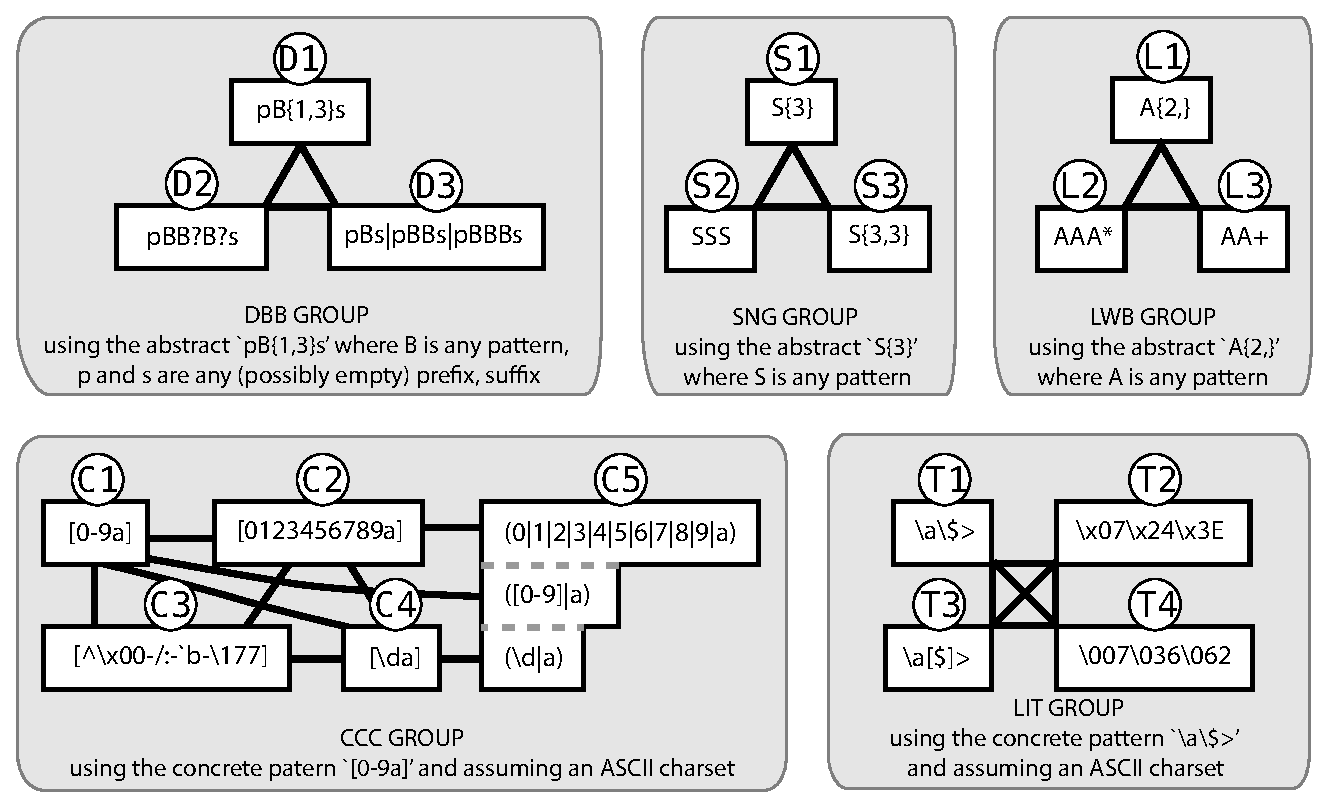
\includegraphics[width=\textwidth]{nontex/illustrations/refactoringTree.eps}
\vspace{-12pt}
\caption{Equivalence classes with various representations of semantically equivalent representations within each class. DBB = Double-Bounded, SNG = Single Bounded, LWB = Lower Bounded, CCC = Custom Character Class and LIT = Literal}
\vspace{-6pt}
\label{fig:refactoringTree}
\end{figure*}

Figure~\ref{fig:refactoringTree} displays five equivalence classes in grey boxes.  This work will often use the term \emph{group} as shorthand for `equivalence class'.  These equivalence classes were chosen by considering what alternatives are possible between the most commonly used features from  Section~\ref{sec:featureResults}.  Three classes focus on representations of repetition (SNG, DBB and LWB), CCC focuses on representations of character classes, and LIT focuses on how characters are represented.  Additional classes of behaviorally identical regexes are discussed in Section~\ref{dis:equivalenceModels}.

Each equivalence class has multiple \emph{nodes} which each represent different ways to express or \emph{represent} the behavior of a particular regex.  Examples of various semantically equivalent \emph{representations} of a regex are shown in white boxes. A \emph{representation} is a particular regex that expresses matching behavior using the style of a particular \emph{node}.

As an example of one equivalence class, consider the LWB group.  Each node in the LWB group has a lower bound on repetitions. Regexes \cverb!A{2,}!, \cverb!AAA*! and \cverb!AA+! are semantically equivalent regexes belonging to the nodes L1, L2 and L3, respectively.
The undirected edges between nodes define possible refactorings.

Figure~\ref{fig:refactoringTree} uses specific examples to more clearly illustrate the characteristics of each node.  However, the \verb!`A'!s in the LWB group abstractly represent any element, and the number of elements is free to vary. The lower bound repetition threshold of 2 provides a useful illustration, but is not meant to describe a requirement for the equivalence class.  The analysis performed for this study uses a lower bound of 1.  Further study is needed on how specific lower bounds, and other variables, may affect preferences among nodes.

\subsubsection{Summary of node membership criteria}
Criteria for node membership is summarized in this section.  For a more detailed description, see Appendix~\ref{app:completeNodeDescriptions}

\begin{description}  \itemsep -1pt
\item[C1:] Any regex using the RNG feature in a CCC like \cverb![a-f]! belongs to C1.
\item[C2:] Any regex that contains at least one CCC without any RNG or defaults like \cverb![aeiou]!belongs to the C2 node.
\item[C3:] Any regex using the NCCC feature like \cverb![^x]! belongs to the C3 node..
\item[C4:] Any regex using a default character class in a CCC like \cverb![\d]! or \cverb![\W]! belongs to the C4 node.
\item[C5:] Any regex containing an OR of length-one sequences (including defaults or other CCCs) like \cverb!(a|\d|x)!belongs to the C5 node.
\end{description}

\begin{description}  \itemsep -1pt
\item[D1:] Any regex that uses the DBB feature, such as \cverb!pB{1,3}s!, belongs to the D1 node.
\item[D2:] Any regex that uses the QST feature like \cverb!xyz?! belongs to D2.
\item[D3:] Any regex that uses OR to express repetition with different upper and lower boundaries like \cverb!pBs|pBBs|pBBBs! belongs to D3..
\end{description}

\begin{description}  \itemsep -1pt
\item[T1:] Patterns using ordinary literal characters, and not belonging to other nodes in the LIT group, like \cverb!a! belong to the T1 node.
\item[T2:] Any regex using hex tokens, such as \cverb!\x07+!, belongs to the T2 node.
\item[T3:]  Any ordinary character wrapped in square brackets so that it becomes a CCC containing exactly one character, like \cverb![x][y][z]! belongs to T3.
\item[T4:] Any regex using octal tokens, such as \cverb!\007!, belongs to the T4 node.
\end{description}

\begin{description}  \itemsep -1pt
\item[L1:] Any regex using the LWB feature like \cverb!A{3,}! belongs to the L1 node.
\item[L2:] Any regex using the KLE feature like \cverb!X*! belongs to the L2 node.
\item[L3:] Any regex using the ADD feature like \cverb!T+! belongs to the L3 node.
\end{description}

\begin{description}  \itemsep -1pt
\item[S1:] Any regex using the SNG feature like \cverb!S{3}! belongs to the S1 node.
\item[S2:] Any regex that is explicitly repeated two or more times, and could use repetition operators, like \cverb!(ab)(ab)! or \cverb!ggg! belongs to the S2 node.
\item[S3:] Any regex with a double-bound in which the lower and upper bounds are same belongs, like \cverb!Z{3,3}! to S3.
\end{description}

\subsubsection{Example regex}
Regexes will often belong to many representations in the equivalence classes described here, and often multiple representations within an equivalence class.
Using an example from a Python project, the regex \cverb![^ ]*\.[A-Z]{3}! is a member of S1, L2, C1, C3, and T1. This is because \cverb![^ ]! maps it to C3, \cverb![^ ]*! maps it to L2, \cverb![A-Z]! maps it to C1, \cverb!\.! maps it to T1, and \cverb![A-Z]{3}! maps it to S1.
As examples of refactorings, moving from S1 to S2 would be possible by replacing \cverb![A-Z]{3}! with \cverb![A-Z][A-Z][A-Z]!.  Moving from L2 to L1 would mean replacing \cverb![^ ]*! with \cverb![^ ]{0,}!, resulting in a refactored regex of: \cverb![^ ]{0,}\.[A-Z][A-Z][A-Z]!.
